%\motto{Use the template \emph{chapter.tex} to style the various elements of your chapter content.}
\chapter{Quanteninformationen}
\label{qbits} % Always give a unique label
% use \chaptermark{}
% to alter or adjust the chapter heading in the running head

\chapterauthor{Burak Demirtas, Dominik Neumaier, Thilo Prünte, Hannes Ringswald, Marvin Rothmann}

\abstract{some abstract}

\section{Der Qubit als Informationsträger}
\subsection{Klassisches Bit vs.\ Qubit}
Ein \emph{Bit} ist die kleinste Informationseinheit in klassischen Computern. Es kann genau einen von zwei Zuständen annehmen:
\[
\text{Bit}\,\in\{0,1\}.
\]
Physikalisch bedeutet das zum Beispiel: Strom an = 1, Strom aus = 0.

Ein \emph{Qubit} ist das Gegenstück im \emph{Quantencomputer}. Anders als ein Bit kann ein Qubit beide Zustände „gleichzeitig“ innehaben – man spricht von \emph{Superposition}. Mathematisch schreiben wir:
\[
\ket{\psi} = \alpha\,\ket{0} \;+\; \beta\,\ket{1}, \quad \alpha, \beta \in \mathbb{C},
\]
wobei \(\alpha\) und \(\beta\) so gewählt werden, dass
\[
|\alpha|^2 + |\beta|^2 = 1.
\]
Die Werte \(|\alpha|^2\) und \(|\beta|^2\) sind die Wahrscheinlichkeiten, das Qubit bei einer Messung in Zustand \(\ket{0}\) bzw.\ \(\ket{1}\) zu finden.

\subsubsection*{Anschaulich als Vektor}
Man kann sich ein Qubit auch als Pfeil in einem Kreis vorstellen. Der Pfeil zeigt auf einen Punkt zwischen „0“ und „1“:

\begin{figure}[H]
  \centering
  \begin{tikzpicture}[scale=2]
    % Achsen
    \draw[->] (0,0) -- (1.2,0) node[right]{$\ket{0}$};
    \draw[->] (0,0) -- (0,1.2) node[above]{$\ket{1}$};
    % Qubit-Pfeil
    \draw[->, thick, blue] (0,0) -- (0.8,0.6)
      node[above right]{$\ket{\psi}$};
    % Hilfslinien
    \draw[dashed, gray] (0.8,0) -- (0.8,0.6);
    \draw[dashed, gray] (0,0.6) -- (0.8,0.6);
  \end{tikzpicture}
  \caption{Qubit als Pfeil im Einheitskreis}
\end{figure}

\subsection{Bloch-Kugel}
Ein Qubit-Zustand lässt sich auch dreidimensional darstellen: als Punkt auf einer Kugel, der \emph{Bloch-Kugel}. Jeder Punkt auf der Oberfläche steht für eine bestimmte Superposition.

\begin{figure}[H]
  \centering
  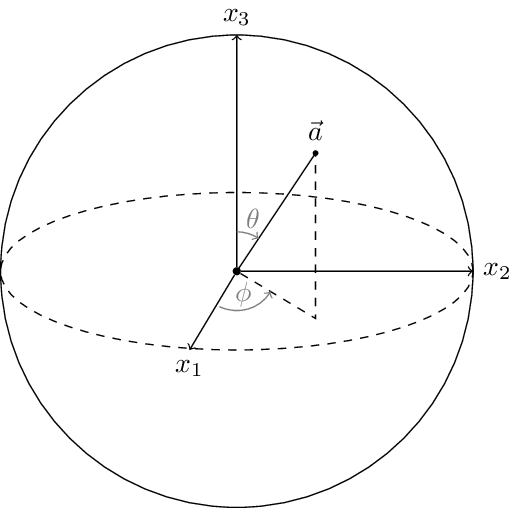
\includegraphics[width=0.7\textwidth]{images/bloch-sphere_quanteninformationen.png}
  \caption{Bloch-Kugel eines Qubits}\label{fig:bloch-sphere}
\end{figure}

Dabei gelten:
\begin{itemize}
  \item Nordpol \(\equiv \ket{0}\)
  \item Südpol \(\equiv \ket{1}\)
  \item Alle anderen Punkte \(\equiv\) Mischzustände aus \(\ket{0}\) und \(\ket{1}\).
\end{itemize}

\subsection{Dirac-Notation kurz erklärt}
In der Quantenmechanik wird die \emph{Dirac-Notation} verwendet:
\begin{itemize}
  \item \(\ket{\psi}\) („Ket“) steht für einen Zustand.
  \item \(\bra{\psi}\) („Bra“) ist die zugehörige Zeile (das „Gegenstück“).
  \item \(\braket{\phi|\psi}\) beschreibt den Überlapp („Skalarprodukt“) zweier Zustände.
\end{itemize}

Beispiele für wichtige Operatoren sind die \emph{Pauli-Matrizen}, die auf ein Qubit wirken:
\[
X=\begin{pmatrix}0&1\\1&0\end{pmatrix},\quad
Y=\begin{pmatrix}0&-i\\i&0\end{pmatrix},\quad
Z=\begin{pmatrix}1&0\\0&-1\end{pmatrix}.
\]

Diese Schreibweise hilft, Rechenregeln in der Quantenmechanik übersichtlich zu formulieren

\subsection{Codierung von Informationen}
\subsubsection{Verschränkung von Qubits}
\subsubsection{Fehlerkorrektur}
\subsubsection{Dense Coding}
%Die fundamentale Funktionsweise klassischer Computer basiert auf einzelnen Bits, welche jeweils den Zustand $0$ (kein Strom) oder $1$ (Strom) annehmen können. Für Berechnungen werden dann Schaltkreise mit Logikgattern verwendet, die zu einer Ausgabe führen. 

%Im Kontext von Quantencomputing ist die kleinste Informationseinheit ein Quantenbit (Qubit). Ein Qubit ist in einer Superposition und kann somit mehr Zustände Annehmen als ein klassisches Bit. %



\section{Quanten-Gatter}\label{sec:quanten_gatter}
Ein Quanten‑Gatter ist eine unitäre Abbildung $U$ auf dem Hilbertraum $\mathcal H \cong (\mathbb C^2)^{\otimes n}$, die - im Gegensatz zu klassischen logischen Operationen - reversibel ist. Da jeder Algorithmus schlussendlich auf eine Folge solcher Unitaries zerlegt werden kann, ist die Auswahl eines
\emph{universellen} Gattersatzes von zentraler Bedeutung.
Aktuelle Experimente realisieren Tor‑Fidelitäten oberhalb von 99{.}999\%, sodass die Schwelle für fehlerkorrigierte Quantenrechnung teilweise bereits überschritten wird.\\

\\
(Vgl. \cite{PhysRevApplied.23.034052}) \\




\subsubsection{Pauli-Gatter $X$, $Y$, $Z$}\label{sec:pauli_gatter}


\paragraph{Hadamard und Superposition}

\paragraph{Matrixdarstellung}



\subsection{Mehr-Qubit-Gatter}

\paragraph{CNOT}



\mathrm{CNOT}=\begin{pmatrix}1&0&0&0\0&1&0&0\0&0&0&1\0&0&1&0\end{pmatrix}

\paragraph{SWAP}





\subsection{Quantenschaltungen}



















\section{Quantenverschränkung und Teleportation}

\subsection{Quantenverschränkung}
Die Quantenverschränkung ist ein Phänomen, bei dem zwei oder mehr Quantenobjekte sich in einem Zustand befinden, in dem sie, egal wie weit voneinander entfernt sie sind, gleich auf externe Reize reagieren. Solche Objekte, bei denen die Quantenverschränkung nachgewiesen werden konnte, sind Atome, Elementarteilchen wie Elektronen und Photonen, bis hin zu Kristallen.\\
\\
An einem Beispiel mit Elektronen lässt sich die Quantenverschränkung wie folgt erklären. Elektronen können sich in einem Zustand befinden, in dem sie keine eindeutige, exakte Position haben, sondern eine Menge an potentiellen Positionen. Diese potentiellen Positionen befinden sich alle im Umfeld der durchschnittlichen Position, dem Massenmittelpunkt des Elektrons, wie eine Wolke. Wenn von diesem Elektron seine Position gemessen wird, antwortet dieses Elektron auf die Messung mit einem zufälligen Wert. Bei den nächsten Messungen wird wiederum mit einem anderen zufälligen Wert geantwortet. Es besteht ein Indeterminismus. In diesem Zustand ist es sogar möglich, dass sich das Elektron, wegen dem Indeterminismus auch an zwei oder mehr Positionen gleichzeitig befindet. Und dieses Elektron, an zwei oder mehr Positionen gleichzeitig, reagiert auf Reize auf die gleiche Weise. Dies wurde im Doppelspaltexperiment von Thomas Young nachgewiesen, bei dem ein Elektron auf einen Reiz an der ersten Position an einem Young‘schen Spalt reagiert, und auf einen Reiz an der zweiten Position an einem anderen Young’schen Spalt reagiert.\\
\\
Obwohl es möglich ist, dass ein Quantenobjekt keine exakte Position hat, und ein weiteres mit dem ersten Quantenobjekt verbundenes, „verschränktes“ Quantenobjekt ebenfalls keine eindeutige Position hat, ist die Distanz zwischen den beiden Quantenobjekten klar bestimmt. Wenn man also die Position der beiden Quantenobjekte misst, erhält man für beide immer einen zufälligen Wert. Aber die Differenz der zufälligen Werte voneinander ist immer genau gleich. Das gilt immer, auch wenn die beiden Quantenobjekte sehr weit voneinander entfernt sind. Die Position eines Quantenobjekts selbst ist nicht wohlbestimmt, die Position im Bezug auf ein verbundenes, verschränktes Quantenobjekt hingegen schon. Dass sich ein Quantenobjekt „hier“ und „einer festen Distanz von hier“ gleichzeitig befindet, wird „Superposition“ genannt. Und dieser superpositionierte Zustand ist ein verschränkter Zustand.\\
\\
Die Verschränkung fixiert nicht nur die Distanz von zwei oder mehr Quantenobjekten voneinander, sondern auch weitere Variablen, z.B. die Geschwindigkeit. Sie haben die gleiche Geschwindigkeit, welche aber selbst nicht fest ist, sondern eine von einer Menge potentieller Geschwindigkeiten.\\
\\
(Vgl. \cite[S.83-88]{gisin_unbegreifliche_2014}) 

\subsection{Quantenteleportation: Protokoll, um einen unbekannten Quantenzustand mithilfe eines verschränkten Paares und klassischer Kommunikation zu übertragen}
Ein Objekt besteht aus Materie und physikalischem Zustand. Bei Quantenobjekten ist die Materie die Masse und permanente Attribute wie z.B. die elektrische Ladung bei Elektronen, bzw. die Energie bei massenlosen Quantenobjekten wie z.B. Photonen. Der physikalische Zustand ist gebildet aus potentiellen Attributen, wie z.B. die potentiellen Positionen (denke Wolke um Massen-/ Energiemittelpunkt), die potentiellen Geschwindigkeiten bei Elektronen bzw. die potentiellen Schwingungsfrequenzen bei Photonen.\\
\\
In der Quantenteleportation wird der Zustand eines Quantenobjekts, der sog. Quantenzustand, ohne das Durchlaufen einer Zwischenstrecke, von einer Position auf eine andere Position, vorausgesetzt, dass sich in dieser anderen Position ein Quantenobjekt derselben Art befindet, direkt versetzt. Die Masse bzw. Energie kann nicht teleportiert werden, weil dies das Prinzip der Unmöglichkeit von Kommunikation ohne Signalübertragung verletzen würde. Dahingegen hat der Zustand weder eine Masse, noch eine Energie, denn sie ist potentiell – eine Wahrscheinlichkeit.\\
\\
Nach einer solchen Quantenteleportation verliert das Quantenobjekt seinen Zustand. Am Beispiel eines Photons kann man dies wie folgt erklären. Es gebe ein Photon mit gut strukturierter Polarisation. Bei solch einem Photon schwingt das elektrische Feld regelmäßig in eine bestimmte Richtung. Nach der Quantenteleportation verliert dieses Photon seine Struktur. Übrig bleibt ein depolarisiertes Photon, ein Photon mit strukturloser Polarisation, dessen elektrisches Feld unregelmäßig in alle Richtungen schwingt. Der Quantenzustand des ersten Quantenobjekts nach der Quantenteleportation entspricht dem Quantenzustand des zweiten Quantenobjekts vor der Quantenteleportation.\\
\\
Der Quantenzustand, der teleportiert wird, ist ein Qubit. Voraussetzung einer Quantenteleportation ist das Dasein einer Menge verschränkter Quantenobjekte. In der nächsten Subsektion wird hierüber genauer erläutert.\\
\\
(Vgl. \cite[S.124-128]{gisin_unbegreifliche_2014}) 


\subsection{Bennett und Brassard (1993): wie drei Qubits (Senderzustand + 2 verschränkte) genutzt werden, um den Zustand über Distanz zu „teleportieren“}
Es gebe ein Quantenobjekt eines Senders mit unbekanntem Quantenzustand bzw. Qubit \(\ket{\Phi}\). Dieser Qubit soll zu einem dritten Quantenobjekt eines Empfängers teleportiert werden. Der Sender ist im Besitz eines zweiten Quantenobjekts mit dem ursprünglichen Zustand \(\ket{\alpha_0}\), „Ancilla“ bzw. „Ancilla-Qubit“ genannt. Im ersten Schritt der Quantenteleportation bringt der Sender das Quantenobjekt mit dem Qubit \(\ket{\Phi}\) und das Quantenobjekt mit dem Ancilla-Qubit dazu, so miteinander zu interagieren, dass das erste Quantenobjekt in einen Standard Zustand \(\ket{\Phi_0}\), und das zweite Quantenobjekt in einen unbekannten Quantenzustand \(\ket{\alpha}\), welches die vollständige Information über \(\ket{\Phi}\) enthält, versetzt wird. Diese Interaktion ist eine gemeinsame Messung der Quantenzustände beider Quantenobjekte des Senders. Allerdings muss erwähnt werden, dass eine solche Messung nur ein positives Ergebnis liefert, wenn der Qubit \(\ket{\Phi}\) einem orthonormalen Set angehört. Im zweiten Schritt der Quantenteleportation wird dann die neue Ancilla, bzw. in anderen Worten das (positive) Ergebnis der Messung im ersten Schritt, an das Quantenobjekt des Empfängers gesendet, wonach der Empfänger die Qubit-Veränderung auslösende Interaktion vom Sender rückgängig machen kann, und somit eine Replikation des originalen Quantenobjekts mit dem Qubit \(\ket{\Phi}\) herstellen kann. Auf dieser Weise können Informationen von Quantenobjekten, also Quanteninformationen, ausgetauscht werden, ohne dass ein Quantenobjekt geklont wird. Diese Methode der Quantenteleportation wird „spin-exchange“ genannt.\\
\\
(Vgl. \cite[S.1-2]{bennett_teleporting_1993})\\
\\
Am anfänglichen Zustand der „spin-exchange“ Methode sind das Quantenobjekt 2 auf der Senderseite und das Quantenobjekt 3 auf der Empfängerseite miteinander verschränkt. Durch die Interaktion auf Senderseite, wobei die Qubits der Quantenobjekte 1 und 2 verändert werden, wird die Verschränkung der Quantenobjekte 2 und 3 aufgehoben, und stattdessen die Quantenobjekte 1 und 2 verschränkt.\\
\\
(Vgl. \cite[S.2-3]{bennett_teleporting_1993})\\
\\
Mathematisch lässt sich der Prozess, wobei die Quantenobjekte in diesem Beispiel spin-\(\frac{1}{2}\) Partikel sind, mit folgenden Formeln darstellen:

\[ \ket{\Psi_{23}^{(-)}} = \sqrt{\frac{1}{2}} (\ket{\uparrow_2}\ket{\downarrow_3} + \ket{{\downarrow_2}\ket{\uparrow_3}}) \]
\\
Das zweite Quantenobjekt vom Sender (2) und das Quantenobjekt vom Empfänger (3) befinden sich in einem verschränkten Zustand. Dies ist die Ausgangssituation.

\[ \ket{\Psi_{12}^{(+)}} = \sqrt{\frac{1}{2}} (\ket{\uparrow_1}\ket{\downarrow_2} + \ket{{\downarrow_1}\ket{\uparrow_2}}) \]
\[ \ket{\Phi_{12}^{(\pm)}} = \sqrt{\frac{1}{2}} (\ket{\uparrow_1}\ket{\uparrow_2} \pm \ket{{\downarrow_1}\ket{\downarrow_2}}) \]
\\
Nun findet die gemeinsame Messung der beiden Quantenobjekte des Senders statt. Die vier sich in den Formeln befindenden Zustände bilden eine orthonormale Basis für die Quantenobjekte 1 und 2. Hiermit ist die Verschränkung der Quantenobjekte 2 und 3 aufgehoben, und stattdessen sind 1 und 2 verschränkt.

\[ \ket{\Phi} = \ket{\Phi_1} = a{\uparrow_1} + b{\downarrow_1} \]
\\
Für einfache Verständlichkeit wird der unbekannte Originalzustand von Quantenobjekt 1, \(\ket{\Phi}\), so geschrieben. Dabei ist \(|a|^2 + |b|^2 = 1\).\\
\\
(Vgl. \cite[S.2]{bennett_teleporting_1993})

\subsection{Quantenkommunikation per Quantenverschränkung in Quantennetzwerken}
In der Quantenkommunikation bzw. im Quanteninformationstransfer innerhalb eines Quantennetzwerks werden Qubits bzw. Quantenzustände über Quantenkanäle gesendet. Quantenkanäle verbinden entfernte Knoten in einem Quantennetzwerk. Diese Quantenkanäle haben eine sog. Absorptionslänge. Die Länge der Quantenkanäle, und damit die maximale Distanz zweier miteinander verbundenen Knoten in einem Quantennetzwerk, ist nur auf wenige Vielfache der Absorptionslänge begrenzt. Dies führt zum Problem, dass Quantenkanäle „eng“ und „laut“ (Originaltext „noisy“) sind, und die transportierten Qubits sich miteinander verschränken können, was zu einem Übertragungsfehler führen könnte.\\
\\
Eine Lösung, die Wahrscheinlichkeit solcher Übertrangungsfehler zu reduzieren, mit Hinnahme von einer größeren Menge an benötigten Ressourcen, ist es, einzelne Qubits in einen konkatenierten Quantencode (z.B. einen verschränkten Zustand einer Vielzahl von Qubits) zu kodieren, und Operationen an diesem Code durchzuführen, während es durch den Quantenkanal übertragen wird. Dies wird „Verschränkungsreinigung“ (vom Eng. „entanglement purification“) genannt und ermöglicht möglichst unverfälschten Quanteninformationstransfer und sichere Quantenkryptographie in „engen“ und „lauten“ Quantenkanälen.\\
\\
Und um unverfälschten Quanteninformationstransfer auch über längere Quantenkanäle sicherzustellen, kann ein Schema verwendet werden, wobei sog. „Quantenrepeater“ einen langen Quantenkanal in kürzere Segmente aufteilen, und die Verschränkungen separat bereinigen, bevor diese wieder aneinander gehängt werden. Im Übergang von einem Segment zum nächsten werden Quantenkorrelationen aufgebaut, basieren auf Korrelationen die innerhalb der einzelnen Segmente existieren.\\
\\
(Vgl. \cite[S.1-2]{dur_quantum_1999})

\subsection{Quantenteleportation in Quantencomputern}
Für folgende Abschnitte gilt die Quelle (Vgl. \cite[S.1-2]{gottesman_quantum_1999}).\\
\\
Die Wissenschaftler Daniel Gottesman und Isaac Chuang stellen eine Technik, eine Verallgemeinerung von Quantenteleportation vor, welche Quantenberechnung in Quantencomputern effizient und ressourcenarm zulässt, und dabei bekannte fehlertolerante Protokolle für Quantenberechnung vereinigt. Mit dieser Technik der Quantenteleportation sollen Quanteninformationen in einen neuen Zustand transformiert werden, was der Wirkung eines Quantengatters ähnelt.\\
\\
Zwei Qubits werden durch ein CNOT (controlled NOT) Gatter (gate) teleportiert. Ein CNOT gate ist eine Komponente, die zwei verschränkte Qubits in einem Bell-Zustand aufnimmt und den zweiten Qubit, den sog. „target“ Qubit dreht, wenn der erste Qubit, der sog. „control“ Qubit, einen Wert von \(\ket{1}\) hat. Beim Durchgang werden Pauli-Matrix Operationen durchgeführt, welche die Quanteninformationen, also den Quantenzustand, auf ein drittes Qubit übertragen.\\
\begin{figure}[h!]
    \centering
    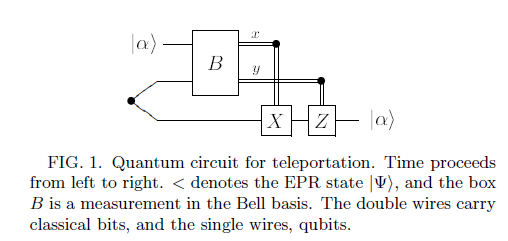
\includegraphics[width=1.0\textwidth]{images/quantenteleportation_cnot_1.png}
    \caption{Zeitstrahl von links nach rechts. B = Bell-Zustand, X Y Z = Pauli Operatoren, \(\ket{\alpha}\) = Zustand des Sender-Qubits, der an den Empfänger-Qubit übertragen werden soll}
    \label{fig:meinbild}
\end{figure}
\newpage
\noindent Dieses Prinzip kann leicht modifiziert werden. Die modifizierte Variante erlaubt es, vier Qubits, wovon jeweils zwei verschränkt sind und sich in einem Bell-Zustand befinden, durchzulassen und anhand von Pauli-Matrix Operationen zu transformieren. Die zwei Bell-Zustand Paare sind vorerst getrennt. Eines beinhaltet den „target“ Qubit \(\ket{\alpha}\), das andere den „control“ Qubit \(\ket{\beta}\). Der „target“ Qubit wird gedreht, wenn der „control“ Qubit einen Wert von \(\ket{1}\) hat. Es stehen 4 Rechenoperationen (I, X, Y, Z) zur Verfügung. Welche Operationen auf die Qubits der Bell-Zustände angewendet werden, ist vom Zufall bestimmt. Was aus dem CNOT gate herauskommt, sind zwei Qubits \(\ket{out}\), welche die Quanteninformationen von \(\ket{\alpha}\) und \(\ket{\beta}\) enthalten, wobei \(\ket{out}\) = CNOT\(\ket{\beta}\)\(\ket{\alpha}\).\\
\begin{figure}[h!]
    \centering
    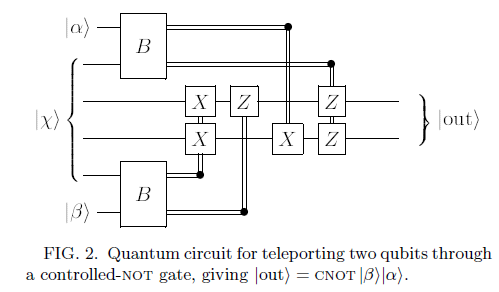
\includegraphics[width=1.0\textwidth]{images/quantenteleportation_cnot_2.png}
    \caption{Zeitstrahl von links nach rechts. B = Bell-Zustand, X Y Z = Pauli Operatoren, \(\ket{\chi}\) = Ausgangszustand für Operation}
    \label{fig:meinbild}
\end{figure}
\newpage
\noindent Eine andere modifizierte Variante ist eine, bei der ein CNOT gate zwischen zwei Qubits von zwei unterschiedlichen verschränkten Qubit Paaren geöffnet wird. Der Output von solch einem Gatter kann verwendet werden, um den Zustand \(\ket{\chi}\) der vorherigen Abbildung zu bilden, von dem in einer Quantenteleportation mit zwei Bell-Zuständen Gebrauch gemacht wird. \(\ket{\chi}\) kann so erzeugt werden, oder durch eine Quantenteleportation zwischen zwei GHZ (Greenberger Horne Zellinger) Zuständen. Ein GHZ Zustand ist eine Verschränkung von drei Quantenobjekten.\\
\begin{figure}[h!]
    \centering
    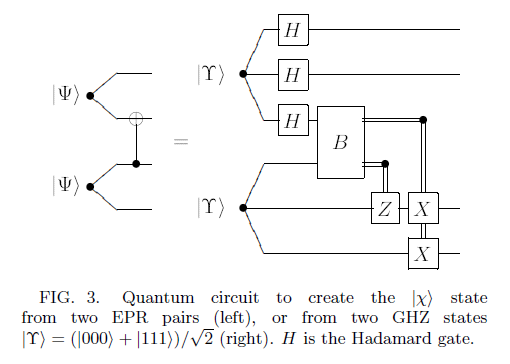
\includegraphics[width=1.0\textwidth]{images/quantenteleportation_cnot_3.png}
    \caption{Zeitstrahl von links nach rechts. \(\ket{\Upsilon}\) = GHZ Zustand, H = Hadamard gate (für Hadamard Transformation), B = Bell-Zustand, X Y Z = Pauli Operatoren}
    \label{fig:meinbild}
\end{figure}
\newpage

\subsection{Bedeutung für Quantenkommunikation und als Demonstration von Quanteninformationstransfer}
Wie Anhand der wissenschaftlichen Artikel von Bennett, Brassard et. al., sowie Gottesmann und Chuang gezeigt wurde, sind Quantenverschränkung und Quantenteleportation die Prinzipien, durch die es zu einem Quanteninformationstransfer kommen kann. Daraus kann man schließen, dass beide Prinzipien eine sehr wichtige Bedeutung für Quantenkommunikation haben.

\section{Praxisbeispiel: Bell-Zustand und Quantenkorrelation}
\subsection{Was ist ein Bell-Zustand?}
Bell-Zustände sind spezielle Zustände in der Quantenmechanik, in denen zwei Teilchen maximal miteinander verschränkt sind. Das bedeutet: Ihre Zustände hängen so stark zusammen, dass man sie nicht unabhängig voneinander beschreiben kann – selbst, wenn die Teilchen physisch weit voneinander entfernt sind. Benannt ist der Bell-Zustand nach dem Physiker John S. Bell. Dieser zeigte im Jahre 1964 auf, dass die Vorhersagen der Quantenmechanik im Widerspruch zu den Prinzipien des lokalen Realismus stehen – also der Vorstellung, dass Informationen nicht schneller als Licht übertragen werden können und physikalische Größen vor der Messung bereits festgelegt sind. (Vgl. \cite[S.195]{bell_einstein_1964})
\\


Mit der von John S. Bell formulierten Bell-Ungleichung entwickelte Bell ein mathematisches Kriterium, mit dem sich klassische und quantenmechanische Theorien experimentell unterscheiden lassen. Die Quantenmechanik sagt unter bestimmten Bedingungen eine Verletzung der nach John S. Bell benannten Bell-Ungleichung voraus. Belegt wurde dies in zahlreichen Experimenten ab 1972, den sogenannten Bell-Test. Seitdem wurde die Verletzung der Bell-Ungleichung in zahlreichen Experimenten mit verschränkten Teilchenpaaren eindeutig nachgewiesen. In allen Fällen bestätigten die Ergebnisse die Vorhersagen der Quantenmechanik. 
(Vgl. \cite[S.53-59]{homeister_quantum_2022})

\subsection{Die vier Bell-Zustände}
Insgesamt existieren vier verschiedene Bell-Zustände, die eine Situation maximaler Verschränkung zwischen zwei Qubits beschreiben. Das heißt: Wird der Zustand eines Qubits gemessen, ist das Ergebnis des anderen automatisch bestimmt. Unabhängig von der Entfernung der Qubits voneinander. (Vgl. \cite[S.53-55]{homeister_quantum_2022}) 
\\


Die vier Bell-Zustände sind nachfolgend dargestellt: 
\[
\begin{aligned}
\ket{\Phi^+} &= \frac{1}{\sqrt{2}} (\ket{00} + \ket{11}), \\
\ket{\Phi^-} &= \frac{1}{\sqrt{2}} (\ket{00} - \ket{11}), \\
\ket{\Psi^+} &= \frac{1}{\sqrt{2}} (\ket{01} + \ket{10}), \\
\ket{\Psi^-} &= \frac{1}{\sqrt{2}} (\ket{01} - \ket{10}).
\end{aligned}
\]

\subsection{Erzeugung eines Bell-Zustands}
Die Erzeugung eines Bell-Zustands basiert auf zwei Schritten. Zu Beginn wird eine Superposition erzeugt, anschließend muss die Verschränkung zwischen den Qubits hergestellt werden. Diese Schritte werden nachfolgend erläutert.
\\


\textbf{Schritt 1 – Superposition erzeugen:} \\
Zuerst wird auf das erste Qubit ein Hadamard-Gatter angewendet. Dadurch wird dieses Qubit in eine Superposition überführt:

\[
\frac{1}{\sqrt{2}} (\ket{0} + \ket{1}) \ket{0} = \frac{1}{\sqrt{2}} (\ket{00} + \ket{10})
\]
\\


\textbf{Schritt 2 – Verschränkung herstellen:} \\
Anschließend folgt ein CNOT-Gatter, bei dem das erste Qubit als Kontroll- und das zweite als Zielqubit fungiert. Dieses Gatter invertiert das Zielqubit nur dann, wenn das Kontrollqubit den Zustand \(\ket{1}\) hat. Dadurch entsteht der Zustand:

\[
\frac{1}{\sqrt{2}} (\ket{00} + \ket{11}) = \ket{\Phi^+}
\]
\\


Es resultiert die vollständige Quantenschaltung zur Erzeugung des Bell-Zustands. Diese ermöglicht es, jeden einfachen Zwei-Qubit-Eingangszustand (\(\ket{00}, \ket{01}, \ket{10}, \ket{11}\)) in einen Bell-Zustand zu überführen.

\begin{figure}[h]
  \centering
  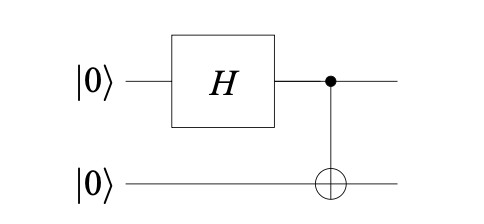
\includegraphics[width=0.6\textwidth]{images/aaf.png}
  \caption{Quantenschaltung zur Erzeugung des Bell-Zustands}
\end{figure}


\\
Es resultiert einer der zuvor vorgestellten Bell-Zustände – ein maximal verschränkter Zustand, in dem die Messungen der beiden Qubits perfekt korreliert sind. Wird in einem verschränkten Bell-Zustand das erste Qubit gemessen, so ergibt sich mit gleicher Wahrscheinlichkeit entweder der Zustand \( \ket{0} \) oder \( \ket{1} \). In beiden Fällen legt diese erste Messung sofort auch den Zustand des zweiten Qubits fest: Beobachtet man \( \ket{0} \) am ersten Qubit, ergibt sich insgesamt der Zustand \( \ket{00} \); misst man \( \ket{1} \), resultiert der Zustand \( \ket{11} \). Eine anschließende Messung des zweiten Qubits führt daher zwangsläufig zum gleichen Ergebnis wie beim ersten – entweder beide Qubits liefern 0 oder beide liefern 1. Je nach Eingangs-Zustand und der Reihenfolge der Gatter ergibt sich ein anderer Bell-Zustand. (Vgl. \cite[S.53-54]{homeister_quantum_2022})
\\


Ein anschauliches Beispiel für die Eigenschaften verschränkter Zustände liefert auch ein Gedankenexperiment mit zwei beispielhaften Personen, Alice und Bob. Angenommen die beiden erzeugten gemeinsam entsprechend der vorhergehenden Ausführungen folgenden Bell-Zustand:
\[
\frac{1}{\sqrt{2}} (|00\rangle + |11\rangle).
\]
Alice erhält nun das erste Qubit, Bob das zweite Qubit. Angenommen die beiden befinden sich ursprünglich in einem Haus im gleichen Raum. Bob nimmt nun sein Qubit mit in ein anderes Zimmer. Solange keine Messung erfolgt und die Qubits vor äußeren Einflüssen geschützt sind, bleibt die Verschränkung erhalten – unabhängig von der räumlichen Trennung. Führt nun einer der beiden eine Messung durch, so ist das Ergebnis zufällig: Mit einer Wahrscheinlichkeit von 50\,\% wird $|0\rangle$ gemessen, mit 50\,\% $|1\rangle$. Erst wenn Alice und Bob ihre Ergebnisse miteinander vergleichen, zeigt sich die Besonderheit: Ihre Messergebnisse stimmen stets überein. Es resultiert eine perfekte Korrelation, unabhängig von Raum und Zeit. (Vgl. \cite[S.54]{homeister_quantum_2022})
\\


Genau darin zeigt sich der Informationsgehalt eines verschränkten Zustands: Die Information liegt nicht in einem einzelnen Qubit, sondern nur in ihrer gemeinsamen Beziehung. Diese Simulation macht das abstrakte Konzept der Quantenverschränkung greifbar und bietet einen intuitiven Zugang zu den Grundlagen der Quanteninformation. Es zeigt anschaulich, wie Quantencomputer fundamentale Prinzipien der Quantenmechanik sichtbar und messbar machen. 

\subsection{Bell-Zustand in der Praxis}

Bell-Zustände bilden das Fundament für viele Anwendungsfälle. Ein praktischer Anwendungsfall ist die Quantenkryptographie. Besonders bekannt ist insbesondere das sogenannte E91-Protokoll, welches auf dem Konzept der Quantenverschränkung beruht. Dabei erzeugt eine zentrale Quelle verschränkte Teilchenpaare und schickt je eines an zwei weit entfernte Personen – wie in unserem Beispiel etwa Alice und Bob. Wenn beide ihre Teilchen messen, erhalten sie stets perfekt korrelierte Ergebnisse. Dieser Effekt lässt sich nutzen, um einen gemeinsamen geheimen Schlüssel zu erzeugen. Ein Abhörversuch durch eine dritte Person würde diese Korrelation stören und könnte über einen Bell-Test erkannt werden. So kann mit Hilfe der Quantenmechanik sichergestellt werden, dass keine unbemerkte Informationsweitergabe stattgefunden hat – eine Grundlage für absolut sichere Kommunikation. (vgl. \cite[S. 3841 f.]{state-of-the-art-survey})
\\


Quantenbasierte Protokolle stehen daher im Zentrum aktueller Forschung zur Quantenkryptographie und wurden bereits in ersten praktischen Experimenten erprobt. Besonders eindrucksvoll ist das Experiment mit dem chinesischen Micius-Satelliten: Er übermittelte verschränkte Photon-Bell-Paare an zwei Bodenstationen, die über eine Entfernung von rund 1200 Kilometern verteilt waren. Die gemessenen Korrelationen verletzten dabei deutlich die Bell-Ungleichung – ein klares Zeichen dafür, dass die beobachteten Effekte nicht durch klassische Physik erklärbar sind, sondern echte Quantenverschränkung vorliegt. Auf dieser Grundlage könnten über Kontinente hinweg geheime Schlüssel erzeugt und die Kommunikation verschlüsselt werden. (vgl. \cite{Entanglement Distribution})
\\


Ein zweiter praktischer Anwendungsfall des Bell-Zustands findet sich im Quantencomputing, genauer gesagt in der sogenannten Quanten-Teleportation. Dabei wird der Zustand eines Quantenbits (Qubit) von einem Ort zu einem anderen übertragen, ohne dass das Teilchen selbst physisch bewegt wird. Grundlage hierfür ist ein gemeinsam genutzter Bell-Zustand zwischen Sender (Alice) und Empfänger (Bob), der die nötige Verschränkung bereitstellt. Durch eine spezielle Messung auf Seiten von Alice und die Übermittlung zweier klassischer Bits kann Bob den ursprünglichen Zustand lokal wiederherstellen. (vgl. \cite{Teleporting}
\\


Im Gegensatz zur Quantenkryptographie, bei der Sicherheit im Vordergrund steht, dient die Quanten-Teleportation der fehlerfreien Übertragung von Quanteninformation. Dies ist eine essenzielle Voraussetzung für die Vernetzung räumlich verteilter Quantencomputer. Sie gilt daher als Schlüsselfunktion zukünftiger Quantencomputer-Netzwerke, etwa im Rahmen eines „Quanteninternets“. (vgl. \cite{Entanglement Distribution}) Erste praktische Umsetzungen konnten dies bereits demonstrieren: 2017 gelang es ein Qubit über 1.400 km mit dem zuvor bereits erwähnten Satellit Micius erfolgreich zu teleportieren. (vgl. \cite{Ground-to-satellite })


\subsection{Simulation mit IBM Quantencomputer}
Die Eigenschaften von Bell-Zuständen lassen sich mithilfe von Quantencomputern, wie denen von IBM, direkt auf Hardware simulieren und beobachten. In diesem Beispiel wurde ein einfacher Quantenschaltkreis aufgebaut, um einen Bell-Zustand zu erzeugen. Ausgangszustand waren zwei Qubits, die beide den Wert 0 hatten. Zunächst wurde auf das erste Qubit ein Hadamard-Gatter (rotes Gatter) angewendet. Dadurch ging es in eine Überlagerung aus „0“ und „1“ über. Anschließend folgte ein CNOT-Gatter (blaues Gatter), das die beiden Qubits miteinander verschränkte: Wenn das erste Qubit auf „1“ übergeht, kippt das zweite automatisch ebenfalls auf „1“. Das Ergebnis ist ein Zustand, in dem die Qubits perfekt miteinander verbunden sind – man spricht von einem verschränkten Zustand. 

\begin{figure}[h]
    \centering
    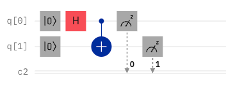
\includegraphics[width=0.5\textwidth]{images/Schaltung_IBM.png}
    \caption{Quantenschaltung - IBM Quantum Learning Platform.}
    \label{fig:meinbild}
\end{figure}

Nach dem Aufbau der Schaltung wurden auf dem IBM-Quantencomputer Messungen durchgeführt. Das bedeutet, dass die Qubits im Z-Basiszustand ausgelesen werden um zu überprüfen, ob sie im Zustand „0“ oder „1“ sind. 

\begin{figure}[ht]
    \centering
    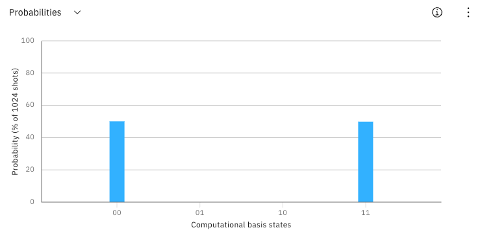
\includegraphics[width=1\textwidth]{images/results_ibm.png}
    \caption{Wahrscheinlichkeitsverteilung - IBM Quantum Learning Platform.}
    \label{fig:meinbild}
\end{figure}


Wie das Histogramm zeigt, wurden ausschließlich die Zustände „00“ und „11“ beobachtet - und zwar mit jeweils rund 50\% Wahrscheinlichkeit. Die Zustände „01“ oder „10“, bei denen sich die beiden Qubits unterscheiden würden, traten gar nicht auf. Dies ist ein typisches Verhalten eines Bell-Zustands und belegt, dass die Qubits verschränkt sind. Bemerkenswert ist dabei: Diese Quantenkorrelation bleibt bestehen, selbst wenn die Qubits räumlich voneinander getrennt wären. Die Messergebnisse des einen beeinflussen scheinbar sofort das andere – ein Verhalten, das mit klassischer Physik nicht erklärbar ist. (Vgl. \cite{Bell State ZZ-Measurement}) 


\printbibliography
